%%%%%%%%%%%%%%%%%%%%%%%%%%%%%%%%%%%%%%%%%%%%%%%%%%%%%%%%%%%%%%%%%%%%%%%%%%%
%% This file is part of the book
%%
%% Algorithmic Graph Theory
%% http://code.google.com/p/graph-theory-algorithms-book/
%%
%% Copyright (C) 2009, 2010, 2011 Minh Van Nguyen <nguyenminh2@gmail.com>
%%
%% See the file COPYING for copying conditions.
%%%%%%%%%%%%%%%%%%%%%%%%%%%%%%%%%%%%%%%%%%%%%%%%%%%%%%%%%%%%%%%%%%%%%%%%%%%

\subfigure[Zachary karate club network.]{
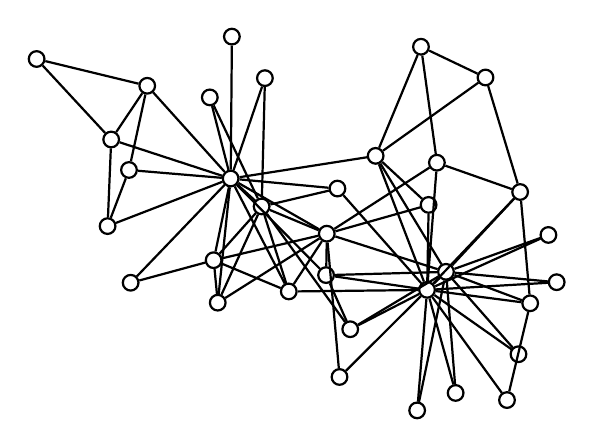
\begin{tikzpicture}
[lineDecorate/.style={-,thick},%
  nodeDecorate/.style={shape=circle,inner sep=2pt,draw,thick},
  scale=1.3,rotate=270]
%% nodes or vertices
\foreach \nodename/\x/\y in {
  0/1.77520000000000/2.16640000000000,
  1/2.04820000000000/2.46890000000000,
  2/2.31390000000000/3.10550000000000,
  3/2.57330000000000/2.00030000000000,
  4/2.24000000000000/0.964260000000000,
  5/0.869150000000000/1.35140000000000,
  6/1.39390000000000/0.999250000000000,
  7/2.98810000000000/2.04030000000000,
  8/2.71860000000000/3.09860000000000,
  9/3.71380000000000/3.23010000000000,
  10/1.69170000000000/1.17320000000000,
  11/0.388890000000000/2.17840000000000,
  12/2.79340000000000/1.18950000000000,
  13/2.87830000000000/2.73430000000000,
  14/3.49170000000000/4.97840000000000,
  15/4.04030000000000/3.98830000000000,
  16/0.607450000000000/0.270830000000000,
  17/0.794510000000000/2.50110000000000,
  18/2.78800000000000/5.35150000000000,
  19/1.87320000000000/3.20980000000000,
  20/2.32650000000000/5.27070000000000,
  21/0.982720000000000/1.96290000000000,
  22/3.87010000000000/4.36440000000000,
  23/1.90680000000000/4.99450000000000,
  24/0.487800000000000/4.02570000000000,
  25/0.788300000000000/4.65610000000000,
  26/3.93940000000000/4.86610000000000,
  27/1.62070000000000/4.18130000000000,
  28/2.03290000000000/4.10000000000000,
  29/2.99420000000000/5.09250000000000,
  30/3.24750000000000/3.33460000000000,
  31/1.55390000000000/3.58310000000000,
  32/2.68670000000000/4.27000000000000,
  33/2.86280000000000/4.08490000000000}
{
  \node (\nodename) at (\x,\y) [nodeDecorate] {};
}
%% edges or lines
\path
\foreach \startnode/\endnode in {
  0/1, 0/2, 0/3, 0/4, 0/5, 0/6, 0/7, 0/8, 0/10, 0/11, 0/12, 0/13, 0/17,
  0/19, 0/21, 0/31, 1/2, 1/3, 1/7, 1/13, 1/17, 1/19, 1/21, 1/30, 2/3,
  2/7, 2/8, 2/9, 2/13, 2/27, 2/28, 2/32, 3/7, 3/12, 3/13, 4/6, 4/10,
  5/6, 5/10, 5/16, 6/16, 8/30, 8/32, 8/33, 9/33, 13/33, 14/32, 14/33,
  15/32, 15/33, 18/32, 18/33, 19/33, 20/32, 20/33, 22/32, 22/33, 23/25,
  23/27, 23/29, 23/32, 23/33, 24/25, 24/27, 24/31, 25/31, 26/29, 26/33,
  27/33, 28/31, 28/33, 29/32, 29/33, 30/32, 30/33, 31/32, 31/33, 32/33}
{
  (\startnode) edge[lineDecorate] node {} (\endnode)
};
\end{tikzpicture}
}
%%
%%
\quad
\subfigure[Linear scaling.]{
\label{fig:Zachary_karate_club:degree_distribution}
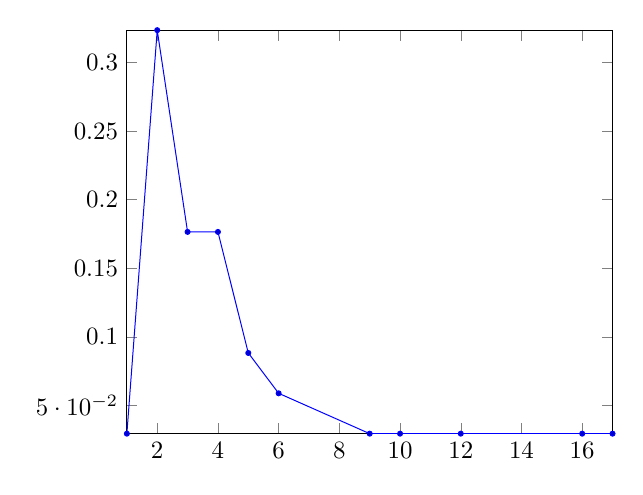
\begin{tikzpicture}
[every mark/.append style={scale=0.5},%
 scale=0.9]
\begin{axis}[%
  enlargelimits=false%
]
\addplot+[sharp plot] coordinates
{
  (1, 0.0294117647058824)  (2, 0.323529411764706)
  (3, 0.176470588235294)   (4, 0.176470588235294)
  (5, 0.0882352941176471)  (6, 0.0588235294117647)
  (9, 0.0294117647058824)  (10, 0.0294117647058824)
  (12, 0.0294117647058824) (16, 0.0294117647058824)
  (17, 0.0294117647058824)
};
\end{axis}
\end{tikzpicture}
}
%%
%%
\subfigure[Log-log scaling.]{
\label{fig:Zachary_karate_club:degree_distribution}
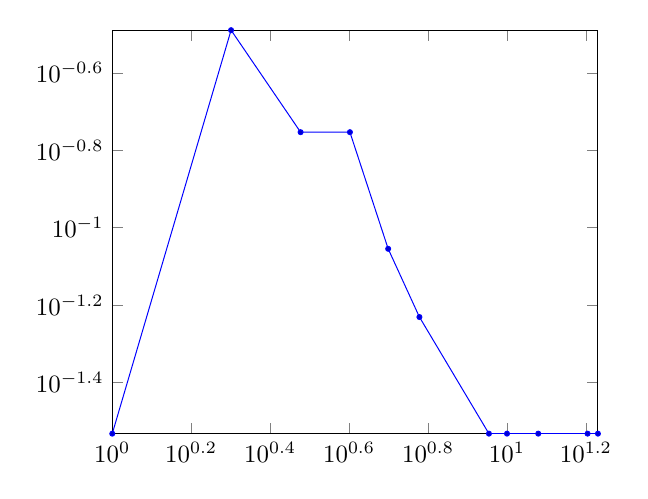
\begin{tikzpicture}
[every mark/.append style={scale=0.5},%
 scale=0.9]
\begin{loglogaxis}[%
  enlargelimits=false%
]
\addplot+[sharp plot] coordinates
{
  (1, 0.0294117647058824)  (2, 0.323529411764706)
  (3, 0.176470588235294)   (4, 0.176470588235294)
  (5, 0.0882352941176471)  (6, 0.0588235294117647)
  (9, 0.0294117647058824)  (10, 0.0294117647058824)
  (12, 0.0294117647058824) (16, 0.0294117647058824)
  (17, 0.0294117647058824)
};
\end{loglogaxis}
\end{tikzpicture}
}
